\documentclass[pdflatex,compress,mathserif]{beamer}

%\usetheme[dark,framenumber,totalframenumber]{ElektroITK}
\usetheme[darktitle,framenumber,totalframenumber]{ElektroITK}

\usepackage[utf8]{inputenc}
\usepackage[T1]{fontenc}
\usepackage{lmodern}
\usepackage[bahasai]{babel}
\usepackage{amsmath}
\usepackage{amsfonts}
\usepackage{amssymb}
\usepackage{graphicx}
\usepackage{multicol}
\usepackage{extarrows}

\newcommand*{\Scale}[2][4]{\scalebox{#1}{$#2$}}%

\title{DIGITAL SIGNAL PROCESSING}
\subtitle{The Discrete Fourier transform}

\author{Mifta Nur Farid}

\begin{document}

\maketitle

\section{Introduction}

\begin{frame}
	\frametitle{Introduction}
	\begin{itemize}
		\item In previous chapters, we have seen how to represent a sequence in terms of a linear combination of complex exponentials using the discrete-time Fourier transform (DTFT) and how the sequence values may be used as the coefficients in a power series expansion of a complex-valued function of $ z $.
		\item For finite-length sequences there is another representation, called the discrete Fourier transform (DFT).
	\end{itemize}
\end{frame}

\begin{frame}{Introduction}
	\begin{itemize}
		\item Unlike the DTFT, which is a continuous function of a continuous variable, $ w $ , the DFT is a sequence that corresponds to samples of the DTFT.
		\item Such a representation is very useful for digital computations and for digital hardware implementations
		\item In this chapter, we look at the DFT, explore its properties, and see how it may be used to perform such tasks as digital filtering and evaluating the frequency response of a linear shift-invariant system.
	\end{itemize}
\end{frame}

\section{Discrete Fourier Series}

\begin{frame}
	\frametitle{Discrete Fourier Series}
	\begin{itemize}
		\item Let $ \tilde{x}(n) $ be a periodic sequence with a period $ N $:
		
		\begin{equation*}
			\tilde{x} = \tilde{x}(n + N)
		\end{equation*}
		
		\item 	Although, strictly speaking, $ \tilde{x}(n) $ does not have a Fourier transform because it is not absolutely summable, it can be expressed in terms of a discrete Fourier series (DFS) as follows:
		
		\begin{equation}\label{6.1}
			\tilde{x}(n) = \frac{1}{N} \sum\limits_{k=0}^{N-1} \tilde{X}(k)e^{j2 \pi nk / N}
		\end{equation}
	
		which is a decomposition of $ \tilde{x}(n) $ into a sum of $ N $ harmonically related complex exponentials.
	\end{itemize}
\end{frame}

\begin{frame}{Discrete Fourier Series}
	\begin{itemize}
		\item The values of the discrete Fourier series coefficients, $ \tilde{X}(k) $, may be derived by multiplying both sides of this expansion by $ e^{-j2\pi nl/N} $, summing over one period, and using the fact that the complex exponentials are orthogonal:
		
		\begin{equation*}
			\sum\limits_{k=0}^{N-1} e^{j2 \pi n (k-l)/N} =
			\begin{cases}
				N & k = l \\
				0 & k \neq l
			\end{cases}
		\end{equation*}
		
		\item The result is
		
		\begin{equation}\label{6.2}
			\tilde{X}(k) = \sum\limits_{k=0}^{N-1} \tilde{x}(n)e^{-j2 \pi n k / N}
		\end{equation}
	\end{itemize}
	 
\end{frame}

\begin{frame}{Discrete Fourier Series}
	
	\begin{itemize}
		\item 	Note that the DFS coefficients are periodic with a period $ N $:
		
		\begin{equation*}
			\tilde{X}(k+N) = \tilde{X}(k)
		\end{equation*}
		
		\item Equations \ref{6.1} and \ref{6.2} form a DFS pair, and we write
		
		\begin{equation*}
			\tilde{x}(n) \xLeftrightarrow{DFT} \tilde{X}(k)
		\end{equation*}
	\end{itemize}
\end{frame}

\begin{frame}
	\frametitle{Example 1}
	\begin{itemize}
		\item Let us find the discrete Fourier series representation for the sequence
		
		\begin{equation*}
			\tilde{x}(n) = \sum\limits_{k=-\infty}^{\infty} x(n-10k)
		\end{equation*}
		
		where
		
		\begin{equation*}
			x(n) =
			\begin{cases}
				1 & 0 \leq n < 5 \\
				0 & \text{else}
			\end{cases}
		\end{equation*}
	\end{itemize}
\end{frame}

\begin{frame}{Example 1}
	\begin{itemize}
		\item Note that $ \tilde{x}(n) $ is a periodic sequence with a period $ N = 10 $. Therefore, the DFS coefficients are
		
		\begin{equation*}
			\tilde{X}(k) = \sum\limits_{n = 0}^9 \tilde{x}(n) e^{-j2 \pi nk / 10} = \sum\limits_{n = 0}^4 e^{-j2 \pi nk / 10} = \frac{1 - e^{-j \pi k}}{1 - e^{-j \pi k/5}}
		\end{equation*}
		
		which, for $ 0 \leq k \leq 9 $ , may be simplified to
		
		\begin{equation*}
			\tilde{X}(k) = \begin{cases}
				5 & k = 0 \\
				\frac{2}{1 - e^{-j \pi k / 5}} & k \text{ odd} \\
				0 & \text{ even}
			\end{cases}
		\end{equation*}
	\end{itemize}
\end{frame}

\begin{frame}{Example 1}
	\begin{itemize}
		\item The DFS coefficients for all other values of $ k $ may be found from the periodicity of $\tilde{X}(k)$:
		
		\begin{equation*}
			\tilde{X}(k + N) = \tilde{X}(k)
		\end{equation*}
		
		\item A notational simplification that is often used for the DFS is to define
		
		\begin{equation*}
			W_N \equiv e^{-j2 \pi /N}
		\end{equation*}
		
		for the complex exponentials and write the DFS pair as follows:
		
		\begin{align*}
			\tilde{x}(n) &= \frac{1}{N}\sum\limits_{k=0}^{N-1}\tilde{X}(k)W_N^{-nk} \\
			\tilde{X}(k) &= \sum\limits_{n=0}^{N-1}\tilde{x}(n)W_N^{nk} \\
		\end{align*}
	\end{itemize}
\end{frame}

\begin{frame}
	\frametitle{The Discrete Fourier Series Properties}
	The discrete Fourier series has a number of useful and interesting properties. A few of these properties are described below.
	\begin{enumerate}
		\item Linearity
		\item Shift
		\item Periodic Convolution
	\end{enumerate}
\end{frame}

\begin{frame}
	\frametitle{Linearity}
	The DFS pair satisfies the property of linearity. Specifically, if $ \tilde{x}_1(n) $ and $ \tilde{x}_2(n) $ are periodic with period $ N $, the	DFS coefficients of the sum are equal to the sum of the coefficients for $ \tilde{x}_1(n) $ and $ \tilde{x}_2(n) $ individually

	\begin{equation*}
		\tilde{x}_1(n) + \tilde{x}_2(n) \xLeftrightarrow{\text{DFS}} \tilde{X}_1(k) + \tilde{X}_2(k)
	\end{equation*}
\end{frame}

\begin{frame}
	\frametitle{Shift}
	If a periodic sequence $\tilde{x}(n)$ is shifted, the DFS coefficients are multiplied by a complex exponential. In other words, if $\tilde{X}(k)$ are the DFS coefficients for $ \tilde{x}(n) $, the DFS coefficients for $ \tilde{y}(n) = \tilde{x}(n - n_0) $ are
	
	\begin{equation*}
		\tilde{Y}(k) = W_N^{kn_0}\tilde{X}(k)
	\end{equation*}

	Similarly, if $\tilde{x}(n)$ is multiplied by a complex exponential,
	
	\begin{equation*}
		\tilde{y}(n) = W_N^{nk_0}\tilde{x}(n)
	\end{equation*}

	the DFS coefficients of $ \tilde{x}(n) $ are shifted:
	
	\begin{equation*}
		\tilde{Y}(k) = \tilde{X}(k + k_0)
	\end{equation*}
\end{frame}

\begin{frame}
	\frametitle{Periodic Convolution}
	If $ \tilde{h}(n) $ and $ \tilde{x}(n) $ are periodic with a period $ N $ with DFS coefficients $ \tilde{H}(k) $ and $ \tilde{X}(k) $, respectively, the sequence
	with DFS coefficients
	
	\begin{equation*}
		\tilde{Y}(k) = \tilde{H}(k)\tilde{X}(k)
	\end{equation*}

	is formed by periodically convolving $\tilde{h}(n)$ with $ \tilde{x}(n) $ as follows:
	
	\begin{equation}
		\tilde{y}(n) = \sum\limits_{k=0}^{N-1} \tilde{h}(k)\tilde{x}(x-k)
	\end{equation}
\end{frame}

\begin{frame}{Periodic Convolution}
	Notationally, the periodic convolution of two sequences is written as
	
	\begin{equation*}
		\tilde{y}(n) = \tilde{h}(n)\circledast\tilde{x}(n)
	\end{equation*}
	
	The only difference between periodic and linear convolution is that, with periodic convolution, the sum is only evaluated over a single period, whereas with linear convolution the sum is taken over all values of $ k $.
\end{frame}

\begin{frame}
	\frametitle{Example 2}
	Let us periodically convolve the two sequences pictured below that have a period $ N = 6 $.
	
	\begin{center}
		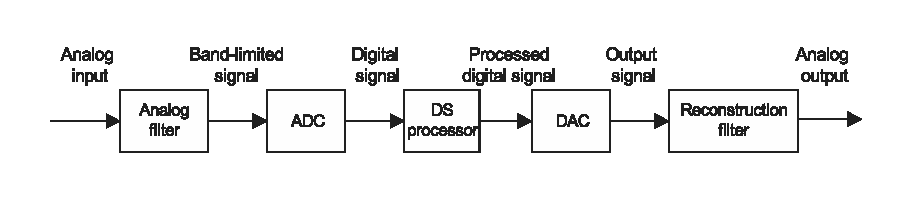
\includegraphics[width=0.7\linewidth]{pic/img01}
	\end{center}
	
\end{frame}

\begin{frame}{Example 2}
	The periodic convolution of two sequences may be performed graphically, analytically, or using the DFS. In this problem,
	we will use the graphical approach. We begin by plotting $ \tilde{x}(n-k) $ versus $ k $. This sequence, for $ n = 0 $. is illustrated below.
	
	\begin{center}
		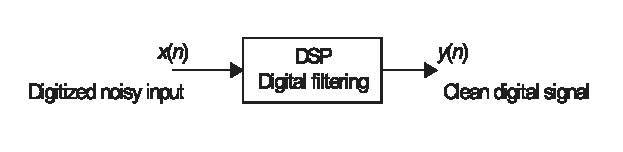
\includegraphics[width=0.7\linewidth]{pic/img02}
	\end{center}

\end{frame}


\begin{frame}{Example 2}
	The value of $ \tilde{y}(0) $ is then found by summing the product $ \tilde{h}(k)\tilde{x}(-k) $ from $ k=0 $ to $ k=5 $. The result is $ \tilde{y}(0) = 1 $. Next, $ \tilde{x} ( - k ) $ is shifted to the right by one and multiplied by $ \tilde{h} ( k ) $. Because the only two nonzero values of $ \tilde{x}(1 - k ) $ are at $ k = 4.5 $, the product $ \tilde{h}(k)\tilde{x}(1 - k ) $ is equal to zero, and $ \tilde{y} ( 1 ) = 0 $ . This process is continued until we have one period of $ \tilde{y}( n ) $ . The result is illustrated below.
	
	\begin{center}
		
\includegraphics[width=0.7\linewidth]{pic/img03}
	\end{center}
\end{frame}

\end{document}
